\chapter{What are Longitudinal Data?}
\makeheading{Week 1}{\daterange{2022-01-05}{2022-01-07}}%chktex 8
\section{What are Longitudinal Data?}
\begin{figure}[H]
    \centering
    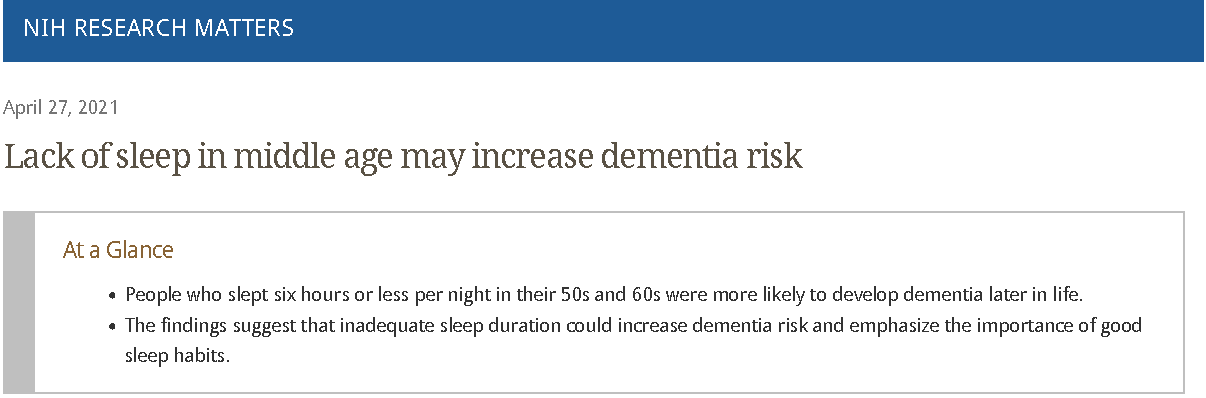
\includegraphics[width=\textwidth]{figures/002-study.pdf}
\end{figure}
What would a study \textbf{need} to look like to conclude this?
\subsection{The Design of a Longitudinal Study}
\begin{itemize}
    \item Can we conclude this by taking a sample of elderly individuals directly?
          \begin{itemize}
              \item \textbf{No}. How do we determine how much they slept 20 years prior?
          \end{itemize}
    \item Can we conclude this by taking a sample of middle-aged individuals directly?
          \begin{itemize}
              \item \textbf{No}. How do we determine who will develop dementia later on?
          \end{itemize}
    \item Can we conclude this by taking independent samples of middle-aged individuals and
          elderly individuals?
          \begin{itemize}
              \item \textbf{No}. How do we pair the individuals?
          \end{itemize}
\end{itemize}
We would \emph{need} to be able to follow individuals, starting when they are middle-aged,
recording information like how often they sleep, and continue following them until the
onset of dementia.
\begin{framed}
    \centering\textbf{This is a longitudinal study}.
\end{framed}
\begin{figure}[H]
    \centering
    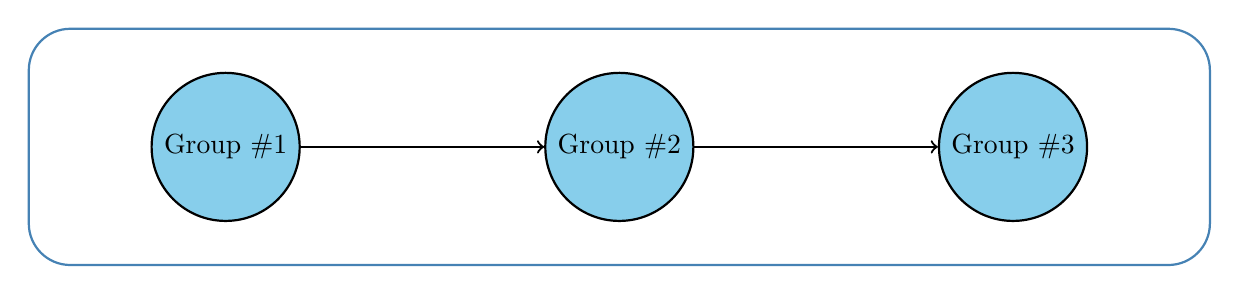
\begin{tikzpicture}[thick]
        \draw[rounded corners=15pt,SteelBlue] (10,0) rectangle ++(15,3);
        \node[draw,circle,fill=SkyBlue] (A) at (12.5,1.5) {Group \#1};
        \node[draw,circle,fill=SkyBlue] (B) at (17.5,1.5) {Group \#2};
        \node[draw,circle,fill=SkyBlue] (C) at (22.5,1.5) {Group \#3};
        \draw[->] (A) -- (B);
        \draw[->] (B) -- (C);
    \end{tikzpicture}
    \caption{Longitudinal Study}
\end{figure}
\begin{figure}[H]
    \centering
    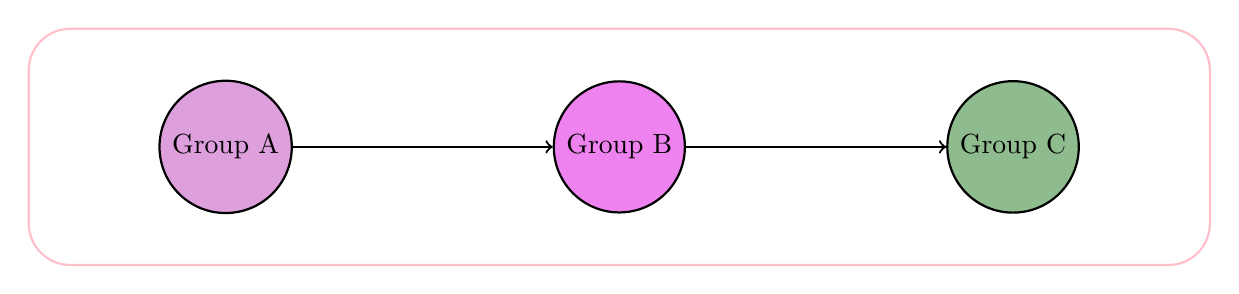
\begin{tikzpicture}[thick]
        \draw[rounded corners=15pt,Pink] (10,0) rectangle ++(15,3);
        \node[draw,circle,fill=Plum] (A) at (12.5,1.5) {Group A};
        \node[draw,circle,fill=Violet] (B) at (17.5,1.5) {Group B};
        \node[draw,circle,fill=DarkSeaGreen] (C) at (22.5,1.5) {Group C};
        \draw[->] (A) -- (B);
        \draw[->] (B) -- (C);
    \end{tikzpicture}
    \caption{Cross-Sectional Study}
\end{figure}
A research study in which \textbf{subjects are followed over time}.
Typically, this involves
repeated measurements of the same variables.
Longitudinal studies differ from \textbf{cross-sectional} studies and
\textbf{time series} studies.
\subsection{Uses for Longitudinal Studies}
\begin{itemize}
    \item To detect changes in outcomes, both at the population and individual level.
    \item \textbf{Longitudinal effects} as compared to \textbf{cohort effects}.
    \item Correctly ascertain the exposures.
    \item Understand different sources of variation
    \item \textbf{Between}- and \textbf{within}-subject variation.
    \item To detect \textbf{time effects}, both directly and as interactions with other relevant
          factors.
\end{itemize}
Bottom line: There are many questions of interest which can only be answered using
longitudinal data. We should probably learn how to analyse it.
\subsection{Why are Longitudinal Data Special?}
What makes longitudinal data more difficult to analyse?
\begin{itemize}
    \item The data are correlated.
    \item Everyone's favourite assumption
          (assume that $ X_1,\ldots,X_n $ are iid) will not hold.
    \item Now what? STAT 437.
\end{itemize}
\subsection{Example Datasets}
\subsubsection{TLC Trial}
\begin{table}[H]
    \centering
    \begin{tabular}{cccccc}
        \toprule
        ID     & Treatment & W0     & W1     & W4     & W6     \\
        \midrule
        1      & P         & 30.8   & 26.9   & 25.8   & 23.8   \\
        2      & A         & 26.5   & 14.8   & 19.5   & 21     \\
        3      & A         & 25.8   & 23     & 19.1   & 23.2   \\
        \vdots & \vdots    & \vdots & \vdots & \vdots & \vdots \\
        98     & A         & 29.4   & 22.1   & 25.3   & 4.1    \\
        99     & A         & 21.9   & 7.6    & 10.8   & 13     \\
        100    & A         & 20.7   & 8.1    & 25.7   & 12.3   \\
        \bottomrule
    \end{tabular}
\end{table}
\begin{itemize}
    \item Is there a difference between \textbf{placebo} and \textbf{treatment}?
    \item How does the blood lead level \textbf{change over time} (in each group)?
    \item Is the \textbf{change} over time \textbf{equal} between treatment groups?
\end{itemize}
\subsubsection{Sales Data}
\begin{table}[H]
    \centering
    \begin{tabular}{ccccc}
        \toprule
        \texttt{DATE} & \texttt{brand} & \texttt{prod} & \texttt{QTY} & \texttt{PROMO} \\
        \midrule
        2014-01-02    & 1              & 1             & 7            & 0              \\%chktex 8
        2014-01-02    & 1              & 2             & 3            & 0              \\%chktex 8
        2014-01-02    & 1              & 3             & 0            & 0              \\%chktex 8
        \vdots        & \vdots         & \vdots        & \vdots       & \vdots         \\%chktex 8
        2018-12-31    & 4              & 8             & 1            & 1              \\%chktex 8
        2018-12-31    & 4              & 9             & 0            & 0              \\%chktex 8
        2018-12-31    & 4              & 10            & 3            & 1              \\%chktex 8
        \bottomrule
    \end{tabular}
\end{table}
\begin{itemize}
    \item Are the \textbf{different brands comparable} in terms of overall sales?
    \item Are the \textbf{different products comparable}?
    \item Do \textbf{promotions increase} the quantity sold? If so, by \textbf{ how much}?
    \item Do the effects of time, and promotion, \textbf{change by brand} or product?
\end{itemize}
\subsubsection{Podcast Data}
\begin{table}[H]
    \centering
    \begin{tabular}{ccccc}
        \toprule
        Rating & No. Reviews & Title                  & Date       & $\cdots$ \\
        \midrule
        4.9    & 6400        & Dissect                & 2019-11-01 & $\cdots$ \\%chktex 8
        4.9    & 26300       & The Adventure Zone     & 2019-11-01 & $\cdots$ \\%chktex 8
        4.8    & 3700        & Song Exploder          & 2019-11-01 & $\cdots$ \\%chktex 8
        \vdots & \vdots      & \vdots                 & \vdots     & \vdots   \\%chktex 8
        4.2    & 1100        & Finding Fred           & 2019-12-01 & $\cdots$ \\%chktex 8
        3.9    & 648         & Inside Frozen 2        & 2019-12-01 & $\cdots$ \\%chktex 8
        4.6    & 6400        & Pop Culture Happy Hour & 2019-12-01 & $\cdots$ \\%chktex 8
        \bottomrule
    \end{tabular}
\end{table}
\begin{itemize}
    \item Can we \textbf{predict} the number of ratings that a podcast will receive over time?
    \item Can we \textbf{predict} the average rating value that a podcast will receive over time?
\end{itemize}
\subsubsection{Stroke Data}
\[ \begin{array}{ccccc}
        \toprule
        \texttt{year} & \text{Prop.}~(0,0) & \text{Prop.}~(0,1) & \text{Prop.}~(1,0) & \text{Prop.}~(1,1) \\
        \midrule
        1             & 57 / 344           & 17 / 72            & 17 / 79            & 5 / 23             \\
        2             & 27 / 287           & 8 / 55             & 9 / 62             & 4 / 18             \\
        3             & 23 / 260           & 8 / 47             & 5 / 53             & 3 / 14             \\
        \vdots        & \vdots             & \vdots             & \vdots             & \vdots             \\
        8             & 10 / 129           & 1 / 15             & 5 / 23             & 1 / 4              \\
        9             & 17 / 119           & 3 / 14             & 4 / 18             & 0 / 3              \\
        10            & 13 / 102           & 1 / 11             & 2 / 14             & 0 / 3              \\
        \bottomrule
    \end{array} \]
\begin{itemize}
    \item This is \textbf{time to event} data.
    \item What is \textbf{probability of surviving} beyond some point?
    \item Does this \textbf{differ} if you previously had a stroke? If you \textbf{received treatment}?
\end{itemize}
\subsection{Summary}
\begin{itemize}
    \item Longitudinal data occur when we take repeated measurements on the same
          individuals over time.
    \item Longitudinal data are required for answering questions about changes within an
          individual (compared to between individuals) and to capture time effects.
    \item Longitudinal data are challenging to work with because the data are correlated.
\end{itemize}